\documentclass[12pt]{article}

\usepackage[onehalfspacing]{setspace}

\usepackage{hyperref}

\usepackage{amsmath}
\usepackage{mathtools}
\usepackage{xfrac}

\usepackage{graphicx}

\usepackage{fullpage}

\usepackage{fancyhdr}
\usepackage{caption}
\usepackage{hhline}

\usepackage{setspace}
\usepackage{textgreek}

\usepackage[backend=bibtex]{biblatex}
\addbibresource{References.bib}

\graphicspath{ {img/} }

\begin{document}

    \begin{titlepage}
    
     \author{
         Tom Bridgwater \and
         Mary O'Donnell \and
         Harapan Ong \and
         Josh Pegman \and
         Mahera Shaikh \and
         Isabella Sharpley \and
         Alex Smith \and
         Esther Uwannah \and
         Tim Yau
     }
     
     \title{The Next High Energy Particle Collider}
     
     \maketitle
     
     \center{
     PHAS3441 - Group 9
          
     Board Member - Dr. Frank Deppisch
     }
    
    \end{titlepage}
 
 \clearpage
 
 \setcounter{tocdepth}{2}
 \tableofcontents
 
 \clearpage
 
 \begin{section}{Executive Summary}
 	
 \end{section}
 
 \begin{section}{Introduction}
 
 \end{section}

 \begin{section}{Basic Particle and Collider Physics}
      \subsection{Introduction}
 
 Particle colliders are particle accelerators which collide two beams charged particles (e.g. quarks, leptons and bosons) or ionic nuclei into each other or a static target. This is achieved by accelerating the particles with electromagnetic fields to kinetic energies in the regions of giga and tera electron volts (velocities in excess of 0.999c). Well known examples are the Large Hadron Collider (LHC) at CERN and the Tevatron at Fermilab.
 
 \subsection{Collision Physics}
 
 \subsubsection{Lepton vs. Hadron Collisions}
 
 Leptons are elementary particles, whereas hadrons are composed of quarks bound via the strong force. Collisions involving hadrons are actually interactions of the constituent quarks and are modelled as such \cite{?}. Evidently the resulting interactions of hadron-hadron will be completely different from lepton-lepton; lepton collisions tend to be considerably cleaner and simpler to analyse \cite{?}.
 
 \subsection{Terms}
 
 \subsubsection{Linear and Circular Colliders}
 
 Colliders can be broken down into two distinct categories, Linear Accelerators (linac) and Circular (ring) Accelerators.
 A linac collides two bunches of particles at a fixed point in the center of a linac. After the intersubsection, the remaining particles can no longer be used since they are travelling in the wrong direction. A ring collider can have multiple collision points along the track (the LHC has four detectors) and after a collision, the uncollided particles continue on to be used again.  
 
 \subsubsection{Beam Energy}
 
 Collisions are at relativistic speeds so the energy is measured in the center of mass frame.
 
 For a fixed target, the collision energy is proportional to the root of E, whereas two beam energy is proportional to 2E and is therefore more efficient \cite{ITP:Energy}.
 
 [Why is higher beam energy better?]
 
 \subsubsection{Luminosity}
 
 Luminosity is a representation of the number of events per unit time and is a measure of the colliders performance. 
 
 $$
 Luminosity = \frac{n N_1 N_2 f}{A}
 $$
 
 n = number of colliding bunches. $N_{1,2}$ = num of particles in each bunch. f = frequency of collisions. A = cross subsectional area of the beam.
 
 [Maximising the luminosity is important to...]
 
 [Compare some luminosity.]
 
 \subsubsection{Synchrotron Radiation}
 
 When charged particles move along a curved path, they emit synchrotron radiation [why/how?]. This detracts from the kinetic energy of the particle and so can impose limits on circular colliders. 
 The amount of energy emitted is inversely proportional to the square of the path radius and proportional to the fourth power of the velocity.  
 Since heavier particles travel slower compared lighter particles with the same kinetic energy, this is a limiting factor for circular colliders of light particles. Accelerating an electron to the same energies as a proton in the LHC would require several orders of magnitude more energy [how much?], hence linacs, which do not lose any energy via synchrotron radiation, are often used for light particle collisions.
 
 Synchrotron radiation is used in research as it is the brightest source of artificial X-Rays.
 
 \subsubsection{Acceleration Gradient}
 
 The acceleration gradient is measure of energy imparted on a particle beam per unit length. For a linac, the particle beam only makes one pass and so the acceleration gradient must be very large to reach the required energies. In comparison, ring colliders can accelerate the particles gradually since they may travel around millions of time before collision. This also allows ring colliders to reach energies an order of magnitude higher than linacs before synchrotron losses become prohibitive.
 
 \subsection{Systems}
 \subsubsection{Radiofrequency Cavities}
 
 RF cavities are used to accelerate the particle beam and are typically spaced along the length of collider \cite{CERN:RFCAV}. Electromagnetic waves 
are contained within the cavity and the resulting EM field transfers energy to passing charged particles. The cavities oscillate at a fixed frequency. A particle arriving at exactly the right time will not be subjected to any force, yet ones ahead or behind will be relatively pulled or pushed to match the ideal velocity. This causes particles to bunch into precise groups. On each pass the bunch will increase in energy.

Klystrons produce EM waves which are fed remotely along a metal waveguide to  the RF cavities. An electron beam is bunched via the same method as a RF cavity and then meets an EM wave at a time where the wave opposes the electron's motion, causing the electrons to slow down and transfer energy to the wave. Klystrons operate with a relatively low current, but voltage in the kilovolt region.
 
 \subsubsection{Beam Control}
 
 Aside from the bunching performed by RF cavities, the particle beam needs to be narrowed in the other two planes and, in a ring collider, bent along the path. A quadrupole arrangement of magnets has two north and two south poles at 90 degrees from each other in a circle pattern and is used for focusing the beam like a lens. The field produced has a minimal potential at the center of the beam, forcing stay particles towards the bunch \cite{Quadrupole}. Dipole magnets are used to bend particles around the path of a ring collider [expand].
 
 
 \subsubsection{Cooling}
 
 Superconductors have an electrical resistance of almost zero. This allows the bending electromagnets to produce extremely strong fields and therefore bend a higher energy particle beam.
 
 Superconducting RF cavities can operate at a higher duty cycle, lower beam impedance (as the apertures can be made wider) and higher efficiency of the RF source (Klystron costs increase exponentially with output). 
 
 The financial savings made from the reduced power requirements during operation is approximately offset by the need to supercool the equipment \cite{?}.
 
 \subsubsection{Storage Rings and Injectors}
 
Many colliders use a mixture of linacs and rings in a chain to gradually raise the particle energy before the beam reaches the collider. These are referred to as booster or injectors. For example, a ring accelerator can be used to increase the energy of leptons with a low acceleration gradient (before synchrotron losses are a consideration) and then send the bunched particles into a linac for higher energy collisions.

Storage rings hold particles at time dilating speeds, this can be useful to store, filter and bunch slow to produce and/or rapidly decaying particles (e.g. antimatter).

 \subsubsection{Detectors}
  
 Detectors are present at the collision point of the particles to observe their momentum, energy and mass. Typically there are several different detectors, each observing a different property. 
 
 Closest to the collision are the tracking devices, which observe the path of the particles by their interference with matter, similar to a cloud chamber. Weakly interacting particles are harder to observe. Momentum can be deduced from the deflection of the particle in a magnetic field. 
 
 Calorimeters then detect energy as particles are forced to deposit their energy into materials. Different materials are stacked in layers for strong and electromagnetic force interactions. 
 
 Velocity of particles, which combined with momentum can determine mass, [TBC - Cherenkov radiation - http://home.web.cern.ch/about/how-detector-works].
 
 Muon detectors are the furthest out, since they need to be large to detect weakly interacting particles.

 \end{section}
 
 \begin{section}{Review of Proposed Colliders}
     \begin{subsection}{ILC}
     
     \end{subsection}
     \begin{subsection}{CLIC}
     
     \end{subsection}
     \begin{subsection}{TLEP}
     
     \end{subsection}
     \begin{subsection}{LHeC}
     
     \end{subsection}
     \begin{subsection}{Muon-Muon}
     
     \end{subsection}
          \subsection{Introduction to $\gamma\gamma$ Colliders}
Photon colliders were originally proposed as potential extensions to linear colliders (there have been designs based on the ILC and CLIC\cite{CLIC:Multilinear}) but can also be built as independent machines. A photon collider operates using the process of inverse Compton scattering\textemdash generating  high energy gamma rays for colliding by directing a low energy laser beam ($\sim$1 eV) into a high energy electron beam (10s of GeV) i.e. the electrons transfer some of their energy to the photons\cite{Chou:Higgs}.

Gamma-gamma ($\gamma\gamma$) collisions result in a large cross section of $\gamma\gamma$ $\rightarrow$ H interactions similar to that in electron-positron colliders, e$^{+}$e$^{-}$ $\rightarrow$ ZH ($\sim$200 fb)\cite{Chou:Higgs} however the energy required for $\gamma\gamma$ collisions is a lot lower\textemdash 80 GeV electron beam energy compared to 120 GeV in the e$^{+}$e$^{-}$ colliders. This reduced energy requirement is beneficial to circular colliders as it corresponds to a decrease in the synchrotron radiation power by a factor of 5 and makes the option of building a circular photon collider at Fermilab named HFiTT\textemdash Higgs Factory in Tevatron Tunnel\textemdash a possibility\cite{Chou:Higgs}. 

The lower energy required for Higgs production makes photon colliders a good option for a new low energy, cost effective Higgs factory. Additional advantages of photon colliders include: no positron source is required, no damping rings, the high polarisation of photons and electrons and the ability to reuse existing infrastructure or extending ones that would be built anyway. However the physics capability of a photon collider is not as wide-ranging as a 240 GeV e$^{+}$e$^{-}$ collider and there are design issues to overcome such as IR optics, power consumption and removal of the spent electrons\cite{Blondel:HiggsF}.
 
\subsubsection{Physics of $\gamma\gamma$-to-Higgs}
A large cross-section of 200 fb is achieved in the direct s-channel $\gamma\gamma$ $\rightarrow$ H reaction. This is an important reaction and enhancement of the signal over the background is achieved for photons of circular polarization in the J=0 state by using a polarized laser\cite{Blondel:HiggsF}.  The CP properties of the Higgs Boson can be measured directly using linearly polarized high-energy photons. In fact photon colliders are the only machines capable of measuring the CP admixture and violation of the Higgs to an accuracy of 1\% or more\cite{Chou:Higgs}.

Photon colliders can measure the H-to-$\gamma\gamma$ partial width ($\gamma\gamma$) to a precision of 1\%\cite{Chou:Higgs}, which is better than any other collider. The $\gamma\gamma$ determines the production rate of Higgs in $\gamma\gamma$ collisions and can be measured by observing the decay mode H $\rightarrow$ bb accounting for ∼57\% of total Higgs decays. In e$^{+}$e$^{-}$− collisions, $\gamma\gamma$ is measured in the H $\rightarrow$ $\gamma\gamma$ decay which has a branching fraction of 0.24\%. Therefore at the photon collider, ``the statistics for the measurement of $\Gamma$(H $\rightarrow$ $\gamma\gamma$) is higher by a factor of $\frac{\frac{0.57}{0.0024}}{4}$ $\simeq$ 60 (and will be even larger if a lower-emmittance electron source becomes available).''\cite{Telnov:Photons} The H-to-$\gamma\gamma$ partial width is an important quantity in Higgs physics because the decay proceeds via an inclusive loop that could reveal heavier particles which the Higgs is unable to directly decay into\textemdash new physics potential.

\subsubsection{SAPPHiRE proposal}
SAPPHiRE (Small Accelerator for Photon-Photon Higgs Production using Recirculating Electrons) is a proposed stand-alone $\gamma\gamma$ collider that presents a cost and time efficient option for a Higgs factory capable of accurately measuring Higgs particle properties. The basic principle of operation in SAPPHiRE is based on the process of inverse compton scattering described above with the collider hitting accelerated electrons with a low energy laser beam ($\sim$3.5 eV) generating a back-scattered gamma beam for collision. By colliding photons, the limits to luminosity arising from beam-beam interactions (beamsstrahlung) of charged particles are avoided\cite{Zimmermann:SAPPHiRE}. The SAPPHiRE collider will be about 9Km in circumference and accelerate particles to 80 GeV thus making it the lowest-energy Higgs factory\cite{Bogacz:SAPPHiRE}.

\subsubsection{Technical design and parameters}                                                                                                            SAPPHIRE's design is based on a pair of $\sim$10 GeV recirculating Linacs, similar to those used for LHeC (the sapphire project emanated from the recirculating linac system at LHEC ). The collider has a Laser back scattering system able to produce a $\gamma\gamma$ peak luminosity of 0.36 × 1034 cm−2 s−1 with ECM ($\gamma\gamma$) ∼ 125 GeV. Hence it will be able to produce tens of thousands of Higgs (H) particles a year in clean experimental conditions\cite{Bogacz:SAPPHiRE}.

\begin{figure}
\centering
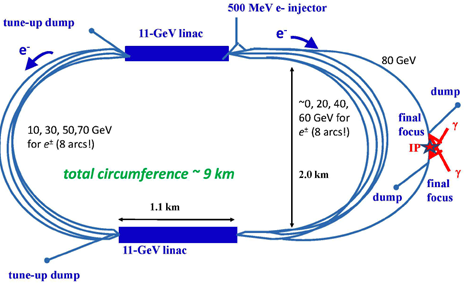
\includegraphics{sapphire1.png}
\caption{Schematic of the SAPPHiRE design based on recirculating superconducting linacs\cite{Bogacz:SAPPHiRE}.}
\end{figure}

The 80 GeV electron beam centre of mass energy required is reached by four passes through the two superconducting recirculating LINACs which increase the electron energy by $\sim$10GeV in each passing.  In comparison to the LHeC, an additional arc is required on both sides with respective beam energies of 70GeV and 80 GeV. The $\gamma\gamma$ collision point is located at the centre of the 80 GeV arc. The Compton scattering point (where gamma beams are generated) is to be located $\sim$1mm from the $\gamma\gamma$ interaction point and laser pulses are required at a frequency of 200kHz. The other laser parameters are: a wavelength of 351nm, 5J pulse energy and a long pulse duration of 5 ps\cite{Bogacz:SAPPHiRE}.

\begin{table}
\begin{center}
\begin{tabular}{l r}
\hline
\hline
Total electric power & 100 MW\\
Beam energy & 80 GeV\\
Beam polarization & 0.80\\
Beam population & $10^{10}$\\
\# of bunches per train & \textemdash\\
\# of trains per rf tube & \textemdash\\
Repetition rate & cw\\
Average bunch frequency & 200 kHz\\
Average beam current & 0.32 mA\\
RMS bunch length & 30 \textmu m\\
Crossing angle & $\geq$ 20mrad\\
Normalised horizontal emittance & 5 \textmu m\\
Nominal horizontal beta function at the IP & 0.5 \textmu m\\
Nominal vertical beta function at the IP & 5 mm\\
Nominal RMS horizontal IP spot size & 400 nm\\
Nominal RMS vertical IP spot size & 18 nm\\
Nominal RMS horizontal CP spot size & 400 nm\\
Nominal RMS vertical CP spot size & 180 nm\\
e$^{-}$e$^{-}$ geometric luminosity & $2.2 \times 10^{34} cm^{-2}s^{-1}$\\
\hline
\hline
\end{tabular}
\caption{Parameters for SAPPHiRE optimised for Higgs mass $\sim$125 GeV}
\end{center}
\end{table}

\subsubsection{Technical feasibility}
The energy loss in an arc is given by:

\begin{equation}
E_{arc}[GeV]=8.846 \times 10^{-5}\frac{(E \ [GeV])^{4}}{2\rho \ [m]}
\end{equation}

Where the bending radius, $\rho$ = 764 m (equal to the LHeC design) and the energy loss in each arc is shown in table 2. Each electron beam loses about 4 GeV in energy, which can be is compensated for by increasing the voltages of the two LINACs from 10 GV to 10.63 GV. The beams in the 70GeV arc lose the most energy due to synchrotron radiation: 1.39 GeV, or a 2\% loss\cite{Bogacz:SAPPHiRE}.

\begin{table}
\begin{center}
\begin{tabular}{c c c}
\hline
\hline
beam energy [GeV] & $\Delta E_{arc}$ [GeV] & $\Delta\sigma_{E}$ [MeV]\\
\hline
10 & 0.0006 & 0.038\\
20 & 0.009 & 0.43\\
30 & 0.05 & 1.7\\
40 & 0.15 & 5.0\\
50 & 0.36 & 10\\
60 & 0.75 & 20\\
70 & 1.39 & 35\\
80 & 1.19 & 27\\
\hline
total & 3.89 & 57 (0.071\%)\\
\hline
\hline
\end{tabular}
\caption{displays the energy losses and energy spread induced in the 8 arcs of SAPPHiRE}
\end{center}
\end{table}

The energy spread from synchrotron radiation in the arc bends is given by:
\begin{equation}
\Delta\sigma^{2}_{E}=\frac{\alpha(\hbar c)^{2}}{48\sqrt{3}}\gamma^{7}\frac{\pi}{\rho^{2}}
\end{equation}

With the geometric radius, R $\simeq$ 1 km and $\rho$ is the dipole bending radius in the arc. The total additional energy spread as a result of synchrotron radiation is only 0.071\%\cite{Bogacz:SAPPHiRE}.

The horizontal emmittance growth of the electron beam caused by synchrotron radiation poses a severe feasibility limitation and is given by:

\begin{equation}
\Delta_{\epsilon/N}=\frac{2pi}{3}\frac{c_{q}r_{e}}{\rho^{2}}\gamma^{6}\langle H \rangle
\end{equation}

Sapphire needs a smaller horizontal emmittance growth than the LHeC which has  = 13 microns at 60GeV.  Reducing the cell length and associated dipole length by a factor of 4 will reduce  at 80GeV to 1 micron, adequate for SAPPHiRE. This means the total length of the bending magnets per optical cell is reduced from $l_{bend}$ $\simeq$ 40 m in the LHeC design to $l_{bend}$ = 10 m for SAPPHiRE\cite{Bogacz:SAPPHiRE}.

Sapphire requires an emmittance ratio of $\frac{\epsilon_{x}}{\epsilon_{y}} \sim 10$, a bunch charge of 1.6 nC and an initial emmittance of $\sim$1.5 \textmu m. These parameters are achievable within the present state of the art. Hence the SAPPHiRE concept employs feasible accelerator parameters. However the main concern is whether we can get polarized beams with these parameters: a polarized low emmittance electron gun is needed. There are ongoing R \& D efforts looking into ``low-emmittance DC guns'' and ``polarized SRF guns.''\cite{Zimmermann:SAPPHiRE}

\subsubsection{Advantages of Sapphire}                                                                                                              The lower beam energy of 80 GeV required to create the Higgs boson allows for efficient recirculation and a 10 times smaller Radio Frequency installation (reducing costs)\cite{Bogacz:SAPPHiRE}. For a stand-alone collider such as the Sapphire, there is no positron beam requirement and no damping rings– further large savings and simplification.

High polarization in the primary electron and the colliding $\gamma$ beams\textemdash in contrast to the case of e$^{+}$\textemdash is becoming a possibility as the Laser technology needed to generate such beams is becoming a reality. SAPPHiRE designs are cost effective (\textless \$1 billion) and take advantage of existing technology and infrastructure. The photon collider concept is applicable to ILC/CLIC as a companion capability. There is no beamstrahlung which results in a higher energy reach than electron positron colliders\cite{Zimmermann:SAPPHiRE}.

\subsubsection{Main issues}
The major design limitation of the SAPPHiRE is the unacceptable increase of horizontal emmittance in the bending arcs: The authors of SAPPHiRE solve this by reducing the dipole section length by 4 which will result in a 64 times smaller emmittance dilution however this requires 16 times stronger quadrupole magnets (quads gradient will be 16 times larger)\cite{Telnov:Photons}.

The initial normalized beam emittances quoted in the sapphire paper of 5 μm and 0.5 μm in the x and y directions respectively, correspond to best unpolarised RF gun emittances but photon colliders need polarised electrons. Currently no low emittance polarized RF guns exist (though progress is being made)\cite{Telnov:Photons:MIT}.

The high-performance laser backscattering system required in collider requires the most R \& D, though money is likely to be made from spin-offs as a result of developments in laser systems which will be beneficial in other fields of science and industry. The main problem is in achieving the lasers high repetition rate of 200kHz; it is possible to overcome this using a passive optical cavity however this is very complex. An alternative approach involves the use of a free electron laser which is cheaper and less complex\cite{Zimmermann:TLEP}.

\subsubsection{Goals and summary of possible measurements}
SAPPHiRE can measure accurately the mass, bb, WW*, and $\gamma\gamma$ decays of the Higgs boson with corresponding plausible statistical errors on these decay paths of 2\%, 5\% and 8\% respectively. In addition, the Higgs mass can be measured to a predicted accuracy of $\sim$100 MeV after 2 years of operation. Other possible decay modes that should be observable include h $\rightarrow$ ZZ* and H $\rightarrow$ Z$\gamma$ but no studies have been made yet. Also, there is the possibility of observing H $\rightarrow$ $\tau^{+}\tau^{-}$ decay\cite{Bogacz:SAPPHiRE}.

CP properties of the H $\rightarrow$ $\gamma\gamma$ partial width can be measured with a precision of about 1\% by taking advantage of both linear and circular polarization, which can't be done at any other collider\cite{Chou:Higgs}.This quantity is of particular interest because the decay proceeds through an inclusive loop that has the potential to reveal heavier charged particles that the Higgs can't directly decay into. The high precision measurements of couplings to standard model particles and possible measurements of non-standard Higgs decays available at SAPPHiRE are beyond the scope of LHC.

\subsubsection{Location and cost}
SAPPHiRE is developed at CERN but could be built elsewhere: it could ``fit" on the SLAC site. Stand-alone photon colliders are compact machines that can be built using existing infrastructure. For example the proposed HFiTT would be located at Fermilab\cite{Chou:Higgs}. It could also be built or as a companion to linear accelerators such as ILC or CLIC. SAPPHIRE's estimated cost $\sim$\$1 billion\textemdash a small fraction of other future projects budgets. 

\subsubsection{Timeline}
Design reports for SAPPHiRE and other proposed photon colliders have not yet been produced. First a conceptual design report will need to be produced followed by a technical design report. 
Taking into account technical readiness, if a stand-alone $\gamma\gamma$ collider such as Sapphire is to be built, it is likely (on a CERN time-scale) to start construction in 2022 with the completion of 5 years of its experimental programme estimated to be sometime between 2030 and 2035. On the other hand if built as an add-on to a linear collider, it would be operational within the active life of e.g. the ILC (2030-2045)\cite{Blondel:HiggsF}.

\subsubsection{Spin-offs}
The generated high energy photon beams have the following characteristics: bright source, monochromatic scattered light (after collimation), tunable wavelength, less expensive than XFEL, broad energy reach (keV, MeV, GeV, TeV) and polarization. Applications of these properties include medical purposes, nuclear material detection and for obtaining polarised e$^{+}$ for e$^{+}$e$^{-}$ linear colliders and many more\cite{Telnov:Overview}.

Spin-offs are likely to be made from the R \& D necessary to create the high-performance laser backscattering system and the polarized RF guns that will be useful in other fields of basic science and industry.

\subsubsection{Conclusion}
SAPPHiRE provides a time and cost effective choice for a Higgs factory. SAPPHiRE can produce the same order of Higgs bosons as an e$^{+}$e$^{-}$ collider and has potential for CP studies and new physics discoveries. However a key issue is the unacceptable increase of the horizontal emittance in the bending arcs. Electron-positron linear colliders can study a greater range of Higgs properties so there is little chance that the physics community will support building SAPPHiRE as the next particle collider instead of e$^{+}$e$^{-}$, and so a photon collider such as SAPPHiRE is best built as an add-on to an e$^{+}$e$^{-}$  collider. Linear colliders are very expensive projects and should be built to maximise the discovery potential therefore considering the relatively low cost of adding a photon collider to a linear collider, a good solution is to combine the two into a collider with two interaction points.

Such an addition at the ILC is conceptually clear but requires enhanced technical design of the laser system. The main thing holding it back is the fact that photon linear colliders need polarized electrons (only in this case can you see the Higgs) and currently low emittance polarized electron guns do not exist.

     \begin{subsection}{SAPPHIRE}
     
     \end{subsection}
 \end{section}
 
 \begin{section}{Comparison of ILC and CLIC}
     \subsection{Introduction}
Although all the colliders we reviewed have their advantages and disadvantages, we have decided to look into two in more depth: ILC and CLIC. 

These colliders have a lot in common. They are both lepton colliders, meaning that they are able to produce clean collisions as the particles do not divide after the collision, and therefore lead to precise measurements. This is in contrast to hadron colliders such as the LHC, which produce collisions in which many particles are released, and are called ‘dirty’ collisions. We have decided to choose lepton colliders, leading to clean collisions, as these are best to determine specific properties of particles such as top, bottom and Z quarks, as well as the Higgs boson. This also allows us to continue the momentum following the discovery of the Higgs boson, by probing it further now that we know its energy level. A lepton collider means that a specific energy range can be chosen, in contrast to colliders such as the LHC where the actual energy range of any collision is can be unknown.

They are also both linear colliders. Although circular colliders such as TLEP can generate large energies, they lose energy to synchrotron radiation, which does not occur with a linear accelerator. This problem could be solved by using a muon collider, as muons have such a small mass that any synchrotron radiation is negligible. However, any plans for muon colliders are far from complete, and the technology needed is unfeasible in the near future. They also both have high maximum energies of 1TeV and 3TeV respectively. This may not seem high in comparison to the 100TeV of the VLHC which consists of TLEP using LHC as an injector; however that project would only begin after the LHC’s lifetime which is a significant amount of time for the scientific community to wait – approximately 40 years.

In addition, ILC and CLIC are the most feasible, as their plans are the most finalised and viable. This is especially true in comparison to colliders such as muon colliders which are completely unfeasible so far and will be for the near future. They use technology which has either already been established or is in the final stages of testing, and they have already found sites to use. They also have plans for funding, whether they are being funded partly by governments, i.e. Japan for ILC, or will be funded by CERN, i.e. CLIC.

\subsection{Cost, feasibility etc.}
 \end{section}
 
 \begin{section}{Conclusion}
 
 \end{section}
 
 \clearpage
 \printbibliography
 
\end{document}
